\documentclass[a4paper,12pt]{article} % тип документа

%  Русский язык
\usepackage[T2A]{fontenc}			% кодировка
\usepackage[utf8]{inputenc}			% кодировка исходного текста
\usepackage[english,russian]{babel}	% локализация и переносы

\usepackage{graphicx}               % импорт изображений
\usepackage{wrapfig}                % обтекаемые изображения
\graphicspath{{pictures/}}          % обращение к подкаталогу с изображениями
\usepackage[14pt]{extsizes}         % для того чтобы задать нестандартный 14-ый размер шрифта
\usepackage{amsfonts}               % буквы с двойными штрихами
\usepackage[warn]{mathtext}         % русский язык в формулах
\usepackage{indentfirst}            % indent first
\usepackage[margin = 25mm]{geometry}% отступы полей
\usepackage{amsmath}                % можно выводить фигурные скобочки -- делать системы уравнений
\usepackage[table,xcdraw]{xcolor}   % таблицы
\usepackage{amsmath,amsfonts,amssymb,amsthm,mathtools} % Математика
\usepackage{wasysym}                % ???
\usepackage{upgreek}                % ???  
\usepackage{caption}
\usepackage{multirow}
\captionsetup{labelsep=period}
\usepackage{gensymb} % degree symbol


\begin{document}
	
	
	\begin{center}
		
		
		\textbf{НАЦИОНАЛЬНЫЙ ИССЛЕДОВАТЕЛЬСКИЙ УНИВЕРСИТЕТ \\ <<МОСКОВСКИЙ ФИЗИКО-ТЕХНИЧЕСКИЙ ИНСТИТУТ>>}
		\vspace{13ex}
		
		\textbf{Лабораторная работа 4.5.1\\ <<Гелий-неоновый лазер>>}
		\vspace{40ex}
		
		\normalsize{Овсянников Михаил Александрович \\ студент группы Б01-001\\ 2 курс ФРКТ\\}
	\end{center}
	
	\vfill 
	
	\begin{center}
		г. Долгопрудный\\ 
		2022 г.
	\end{center}
	
	
	\thispagestyle{empty} % выключаем отображение номера для этой страницы
	\newpage
	
	
	\textbf{Цель работы:} изучение основных принципов работы газового лазера и свойств лазерного излучения.
	
	
	\textbf{В работе используются:} юстировочный лазер, гелий-неоновая трубка, компьютер со звуковой картой, модулятор (обтюратор), фотодиоды, зеркала, поляроид.
	
	\section*{Теоретические сведения}
	
	Главными элементами практически любого лазера являются два параллельных друг другу зеркала и расположенная между ними среда, усиливающая свет. Усиление света основано на явлении вынужденного излучения, которое является обратным поглощению света. Как известно из опыта, при поглощении электромагнитного излучения веществом атомы или молекулы, находящиеся на каком-либо энергетическом уровне, переходят на более высокий свободный уровень, поглощая один квант (фотон) излучения. Поглощение возникает только в том случае, если энергия фотона совпадает с разницей энергий между этими уровнями. Явление вынужденного излучения заключается в том, что если атом находится на возбужденном уровне, то под действием электромагнитного поля происходит обратный переход с возбужденного уровня на более низкий уровень с излучением кванта света.
	
	\begin{figure}[h!]
		\centering
		\includegraphics[scale=0.55]{Pictures/Схема Лазера}
		\caption{Схема лазера}
	\end{figure}

	Рассмотрим механизм возникновения усиления в рабочей среде гелий-неонового лазера. Лазерная трубка заполняется смесью гелия и неона в соотношении от 5:1 до 10:1 с общим давлением порядка 10$^2$ Па, при котором довольно легко возбудить постоянный электрический разряд. Рабочим лазерным веществом является неон. Гелий используется для избирательного заселения верхнего рабочего уровня неона. Атомы гелия возбуждаются при столкновениях с разогнанными в электрическом поле разряда электронами. Передача энергии от возбужденных атомов гелия к атомам неона осуществляется при столкновениях между ними. Известно, что наиболее эффективно передача энергии от атома к атому происходит в резонансном случае, то есть когда энергии уровней, между которыми происходит переход, близки. Упрощенная схема энергетических уровней атомов гелия и неона изображена на рисунке 2.
	
	\begin{figure}[h!]
		\centering
		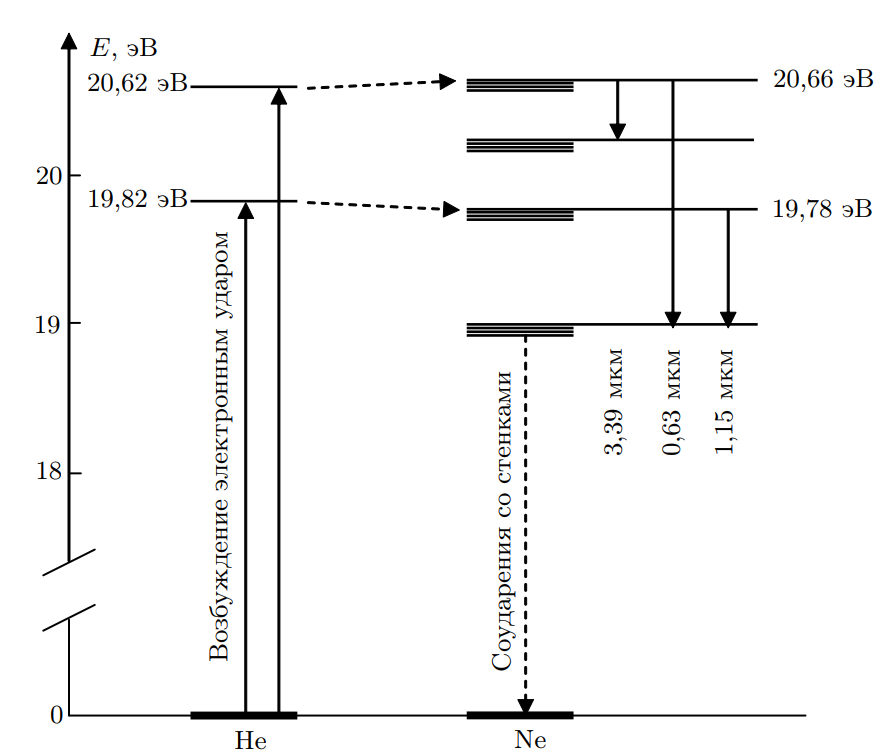
\includegraphics[scale=0.6]{Pictures/Переход}
		\caption{Энергетическая схема работы гелий-неонового лазера}
	\end{figure}
	
	\newpage
	\section*{Экспериментальная установка}
	
	\begin{figure}[h!]
		\centering
		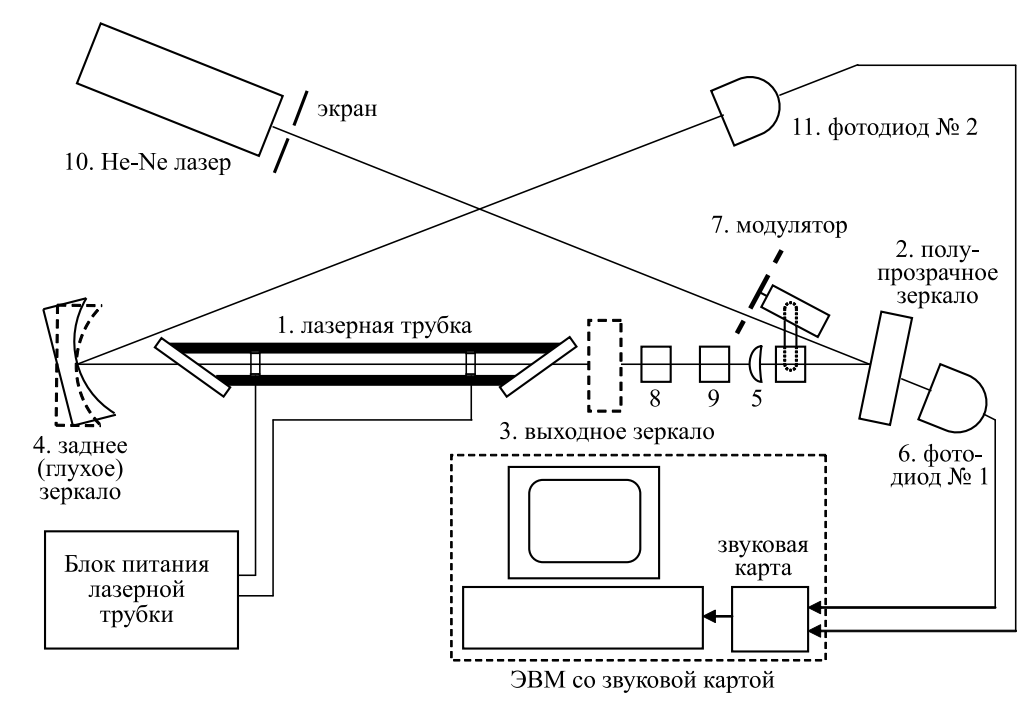
\includegraphics[scale=0.7]{Pictures/Установка}
		\caption{Экспериментальная установка}
	\end{figure}

	Схема экспериментальной установки приведена на рис. 3. На оптической скамье расположены: газоразрядная трубка исследуемого He-Ne лазера ЛГ-75 (1), рейтера для крепления юстировочных оправ с зеркалами (2, 3, 4), линза, уменьшающая расходимость юстировочного лазера (5), фотодиод (6), модулятор (7) а также съемный рейтер (8) с отрицательной линзой для наблюдения модовой структуры излучения исследуемого лазера и рейтер (9), в который вставляется либо экран, либо поляроид. Юстировочный лазер (10) и фотодиод (11) закреплены на столе. Юстировочный лазер предназначен для юстировки всех элементов установки и для измерения коэффициента усиления активной среды исследуемого лазера.
	
	Поскольку коэффициент усиления на рабочей частоте лазера мал, и усиление интенсивности луча зондирующего лазера при длине трубки $\approx 1$ м составляет всего несколько процентов, в данной работе измеряется одновременно интенсивность излучения до и после прохождения исследуемой среды.
	
	\newpage
	\section*{Ход работы}
	
	Включим вилку питания юстировочного лазера в сеть и убедимся в наличии лазерного излучения. Проведем юстировку оптической схемы установки.
	
	\begin{center}
		\textbf{I. Исследование модовой структуры}
	\end{center}
	
	Для начала пронаблюдаем строение модовой структуры лазерного излучения. Поставим на рельс вплотную к выходному зеркалу рейтер с короткофокусной линзой а в рейтер (9) вместо поляроида вставим белый экран. Наблюдая за пятном излучения лазера, с помощью малого поворота одного зеркала получим двухмодовый, трёхмодовый и многомодовый режимы.
	
	Наблюдаем следующие картины:
	
	\begin{figure}[h!]
		\centering
		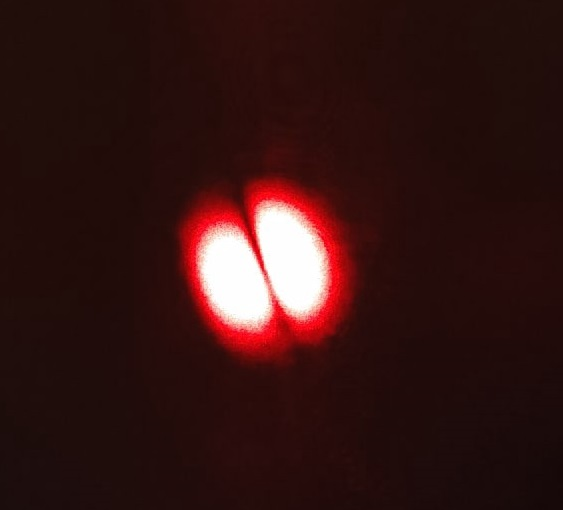
\includegraphics[scale=1.2]{Pictures/Двухмодовый}
		\caption{Двухмодовый режим лазера}
	\end{figure}

	\newpage
	
	\begin{figure}[h!]
		\centering
		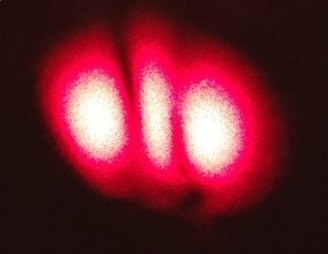
\includegraphics[scale=1.9]{Pictures/Трехмодовый}
		\caption{Трехмодовый режим лазера}
	\end{figure}

	\begin{figure}[h!]
		\centering
		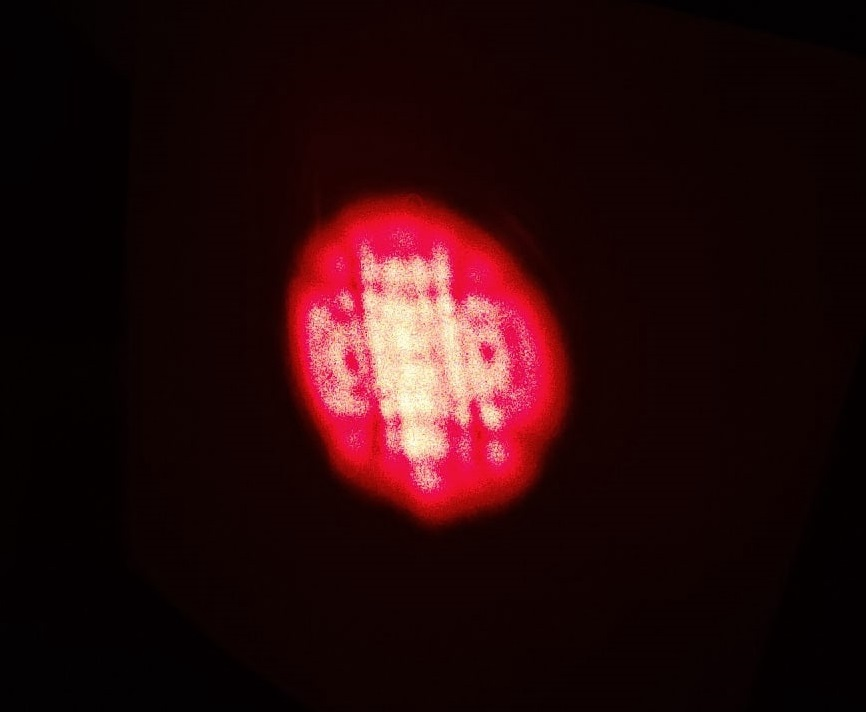
\includegraphics[scale=0.72]{Pictures/Многомодовый}
		\caption{Многомодовый режим лазера}
	\end{figure}

	\newpage

	\begin{center}
		\textbf{II. Изучение поляризации лазерного луча}
	\end{center}
	
	Закрепим в рейтере (9) перед выходным зеркалом поляроид. Повернем и настроим фотодиод и модулятор так, чтобы пучок исследуемого лазера хорошо проходил сквозь отверстия модулятора и попадал на фотодиод (6). Измерим зависимость интенсивности излучения, то есть показаний компьютера, исследуемого лазера в зависимости от угла поворота поляроида. Результаты занесем в таблицу 1:
	
	\begin{table}[h!]
		\centering
		\begin{tabular}{|c|c|c|}
			\hline
			Поворот поляризатора $\theta ^\circ$ & Показания компьютера $U_{\text{эф}}$, мВ & $\sigma_{U_{\text{эф}}}$, мВ \\ \hline
			0                                          & 14,9                                     & 0,2                         \\ \hline
			20                                         & 18,5                                     & 0,5                         \\ \hline
			40                                         & 19,8                                     & 0,2                         \\ \hline
			60                                         & 17,5                                     & 0,1                         \\ \hline
			80                                         & 10,4                                     & 0,1                         \\ \hline
			100                                        & 3,5                                      & 0,1                         \\ \hline
			120                                        & 1,9                                      & 0,1                         \\ \hline
			140                                        & 2,5                                      & 0,1                         \\ \hline
			160                                        & 7,3                                      & 0,1                         \\ \hline
			180                                        & 14,1                                     & 0,3                         \\ \hline
			200                                        & 20,5                                     & 0,2                         \\ \hline
			220                                        & 20,6                                     & 0,2                         \\ \hline
			240                                        & 18,8                                     & 0,2                         \\ \hline
			260                                        & 11,9                                     & 0,1                         \\ \hline
			280                                        & 4,3                                      & 0,1                         \\ \hline
			300                                        & 1,8                                      & 0,1                         \\ \hline
			320                                        & 2,5                                      & 0,1                         \\ \hline
			340                                        & 7,9                                      & 0,1                         \\ \hline
		\end{tabular}
	\caption{Характер поляризации лазерного излучения}
	\end{table}

	\newpage

	Построим зависимость относительной интенсивности от угла поворота поляроида.
	
	\begin{figure}[h!]
		\centering
		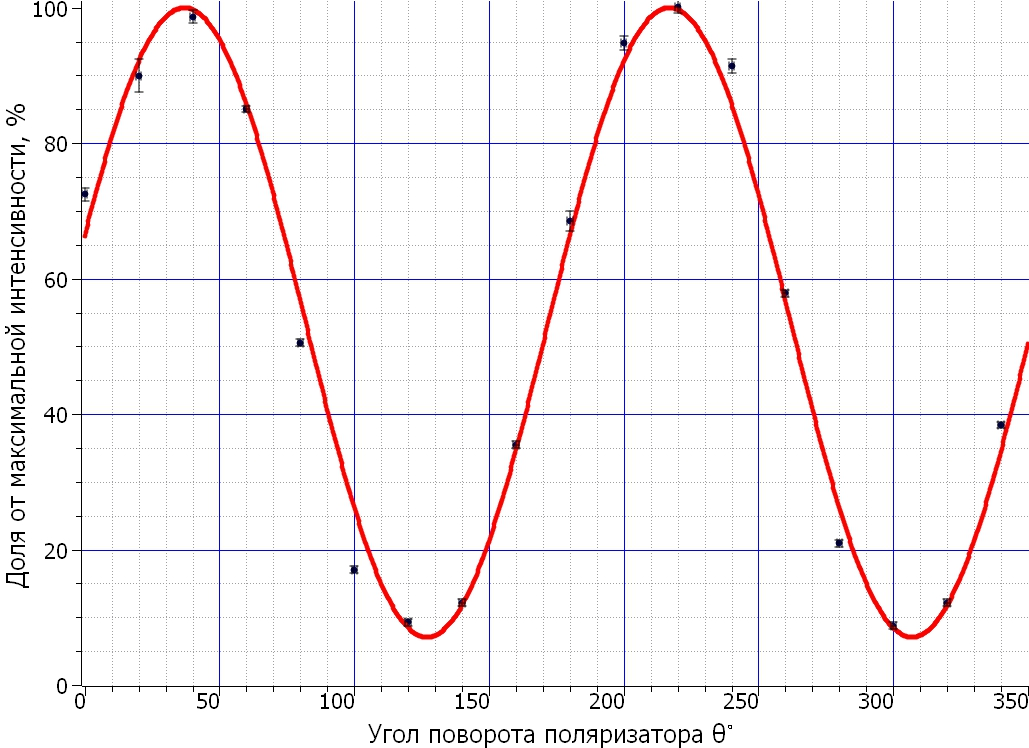
\includegraphics[scale=0.7]{Pictures/Поляризация}
		\caption{Зависимость относительной интенсивности от угла поворота}
	\end{figure}

	Видно, что зависимость являет собой синусоиду. Однако она не достигает нуля -- следствие того, что осциллограф компьютера недостаточно откалиброван.
	
	Наибольшее значение интенсивности лазерного излучения достигается при углах $\theta \thicksim 38 ^\circ + 180^\circ \cdot k, \; k\in \mathbb{Z}$.

	\begin{center}
		\textbf{III. Определение коэффициента усиления среды}
	\end{center}

	Теперь исследуем самое главное -- а именно коэффициент усиления среды.
	
	Включим питание исследуемого и юстировочного лазеров. Запустим осциллограф, включим режим вывода эффективных значений напряжения по обоим каналам и выберем скорость развёртки 1 мс/дел, а ее длительность -- 500 мс для наибольшей точности. Поделив отношения сигналов с  включенным и выключенным питанием трубки друг на друга, получим коэффициент усиления $G$.
	
	
	\newpage 
	С выключенным питанием получаем:
	
	$U_{\text{эф}_1} = (53,5 \pm 0,1)$ мВ; $\hspace{40mm} U_{\text{эф}_2} = (96,0 \pm 0,2)$ мВ.
	
	При включенной трубке получаем следующие значения при разных токах:
	
	\begin{table}[h!]
		\centering
		\begin{tabular}{|c|c|c|}
			\hline
			$I$, мА & $U_{\text{эф}_1}$, мВ & $U_{\text{эф}_2}$, мВ \\ \hline
			46      & 54,2 $\pm$ 0,2        & 94,8 $\pm$ 0,2        \\ \hline
			29      & 55,2 $\pm$ 0,2        & 95,8 $\pm$ 0,3        \\ \hline
			21      & 56,0 $\pm$ 0,2        & 97,3 $\pm$ 0,3        \\ \hline
		\end{tabular}
		\caption{Показания при включенной трубке}
	\end{table}

	Учитывая, что
	\begin{equation*}
		G = \left(\frac{U_{\text{эф}_1}}{U_{\text{эф}_2}}\right)^{\text{вкл}} \Bigg/ \;\left(\frac{U_{\text{эф}_1}}{U_{\text{эф}_2}}\right)^{\text{выкл}}, 
	\end{equation*}

	\noindent то:
	
	\begin{equation*}
		\sigma_G = G\sqrt{
			\left(\frac{\sigma_{U_{\text{эф}_1}^{\text{вкл}}}}{U_{\text{эф}_1}^{\text{вкл}}}\right)^2 + \left(\frac{\sigma_{U_{\text{эф}_2}^{\text{вкл}}}}{U_{\text{эф}_2}^{\text{вкл}}}\right)^2 + \left(\frac{\sigma_{U_{\text{эф}_1}^{\text{выкл}}}}{U_{\text{эф}_1}^{\text{выкл}}}\right)^2+ \left(\frac{\sigma_{U_{\text{эф}_2}^{\text{выкл}}}}{U_{\text{эф}_2}^{\text{выкл}}}\right)^2}
	\end{equation*}

	И тогда таблица 2 приобретает такой вид:
	
	\begin{table}[h!]
		\centering
		\begin{tabular}{|c|c|c|}
			\hline
			$I$, мА & $G$               & $(G - 1) \cdot 10^{-3}$ \\ \hline
			46      & 1,026 $\pm$ 0,005 & 26 $\pm$ 5              \\ \hline
			29      & 1,034 $\pm$ 0,006 & 34 $\pm$ 6              \\ \hline
			21      & 1,033 $\pm$ 0,006 & 33 $\pm$ 6              \\ \hline
		\end{tabular}
	\caption{Итоговые результаты для коэффициента усиления среды}
	\end{table}

	Отчетливо видно, что все три значения, полученные при разных токах, очень близки друг к другу. Также, замечательно то, что все три значения $G \thickapprox$ 1,03. То есть усиление составляет около 3\% за проход! 

	\newpage
	\begin{center}
		\textbf{IV. Настройка лазера на генерацию}
	\end{center}

	Проведем настройку исследуемого лазера для получения генерации.
	\begin{enumerate}
		\item Сначала настроим заднее сферическое зеркало, выходное зеркало при этом снято. Пучок, прошедший через трубку, задним зеркалом направляется строго обратно так, чтобы после вторичного прохождения через трубку исследуемого лазера он попал на экран, закреплённый на выходном торце зондирующего лазера.
		
		\item Поставим на скамью перед трубкой рейтер с выходным зеркалом, рабочей поверхностью к исследуемому лазеру. Это зеркало юстируем так, чтобы отраженный от него луч зондирующего лазера попал в то же самое место, куда попадал пучок, отраженный от сферического заднего зеркала.
		
		\item Включим блок питания исследуемого лазера. Когда загорится разряд, появляется генерация, которую мы определим по появлению ярких красных пятен на зеркалах.
		
		\item Тонкой подстройкой зеркал добьемся максимальной мощности генерации.
	\end{enumerate}  


	\vspace{30mm}
	\section*{Вывод}
	В данной работе мы изучили основные принципы работы газового лазера и свойства лазерного излучения на примере гелий-неонового лазера. Сперва мы пронаблюдали его модовый состав. Затем был выявлен характер поляризации излучения, и было выяснено, что максимум приходится на углы $38^\circ$ и $218^\circ$ поляризатора. Главным достижением работы стало исследование коэффициента усиления среды, сквозь которую проходит лазерного излучение. Значение данного коэффициента составляет $G$ = (1,033 $\pm$ 0,006). То есть за проход усиление составляет $\thickapprox 3\%$! Это достаточно немало для лабораторного лазера. Однако есть погрешности измерений, которые приводят к небольшим ошибкам и неточностям -- они составляют $\thicksim 15-20\%$. Они связаны с несовершенством техники измерения. 
\end{document}